\documentclass[]{report}
\usepackage{amsmath,amssymb}
\usepackage{lmodern}
\usepackage[T1]{fontenc}
\usepackage{amsmath,amssymb}
\usepackage{lmodern}
\usepackage[french]{babel}
\usepackage{setspace}
\usepackage{xcolor}
\usepackage[headheight=13pt,top=3cm, bottom=2cm, left=1cm, right=1cm]{geometry}
\usepackage{fancyhdr}
\pagestyle{fancy}
\usepackage{hyperref}
\usepackage{wrapfig}
\hypersetup{
    colorlinks=true,
    linkcolor=black,
    citecolor=black,
    filecolor=black,
    urlcolor=black,
}
\usepackage{iftex}
\ifPDFTeX
  \usepackage[T1]{fontenc}
  \usepackage[utf8]{inputenc}
  \usepackage{textcomp} % provide euro and other symbols
\else % if luatex or xetex
  \usepackage{unicode-math}
  \defaultfontfeatures{Scale=MatchLowercase}
  \defaultfontfeatures[\rmfamily]{Ligatures=TeX,Scale=1}
\fi
% Use upquote if available, for straight quotes in verbatim environments
\IfFileExists{upquote.sty}{\usepackage{upquote}}{}
\IfFileExists{microtype.sty}{% use microtype if available
  \usepackage[]{microtype}
  \UseMicrotypeSet[protrusion]{basicmath} % disable protrusion for tt fonts
}{}
\makeatletter
\@ifundefined{KOMAClassName}{% if non-KOMA class
  \IfFileExists{parskip.sty}{%
    \usepackage{parskip}
  }{% else
    \setlength{\parindent}{0pt}
    \setlength{\parskip}{6pt plus 2pt minus 1pt}}
}{% if KOMA class
  \KOMAoptions{parskip=half}}
\makeatother
\usepackage{xcolor}
\IfFileExists{xurl.sty}{\usepackage{xurl}}{} % add URL line breaks if available
\IfFileExists{bookmark.sty}{\usepackage{bookmark}}{\usepackage{hyperref}}
\hypersetup{
  hidelinks,
  pdfcreator={LaTeX via pandoc}}
\urlstyle{same} % disable monospaced font for URLs
\usepackage{color}
\usepackage{fancyvrb}
\newcommand{\VerbBar}{|}
\newcommand{\VERB}{\Verb[commandchars=\\\{\}]}
\DefineVerbatimEnvironment{Highlighting}{Verbatim}{commandchars=\\\{\}}
% Add ',fontsize=\small' for more characters per line
\newenvironment{Shaded}{}{}
\newcommand{\AlertTok}[1]{\textcolor[rgb]{1.00,0.00,0.00}{\textbf{#1}}}
\newcommand{\AnnotationTok}[1]{\textcolor[rgb]{0.38,0.63,0.69}{\textbf{\textit{#1}}}}
\newcommand{\AttributeTok}[1]{\textcolor[rgb]{0.49,0.56,0.16}{#1}}
\newcommand{\BaseNTok}[1]{\textcolor[rgb]{0.25,0.63,0.44}{#1}}
\newcommand{\BuiltInTok}[1]{#1}
\newcommand{\CharTok}[1]{\textcolor[rgb]{0.25,0.44,0.63}{#1}}
\newcommand{\CommentTok}[1]{\textcolor[rgb]{0.38,0.63,0.69}{\textit{#1}}}
\newcommand{\CommentVarTok}[1]{\textcolor[rgb]{0.38,0.63,0.69}{\textbf{\textit{#1}}}}
\newcommand{\ConstantTok}[1]{\textcolor[rgb]{0.53,0.00,0.00}{#1}}
\newcommand{\ControlFlowTok}[1]{\textcolor[rgb]{0.00,0.44,0.13}{\textbf{#1}}}
\newcommand{\DataTypeTok}[1]{\textcolor[rgb]{0.56,0.13,0.00}{#1}}
\newcommand{\DecValTok}[1]{\textcolor[rgb]{0.25,0.63,0.44}{#1}}
\newcommand{\DocumentationTok}[1]{\textcolor[rgb]{0.73,0.13,0.13}{\textit{#1}}}
\newcommand{\ErrorTok}[1]{\textcolor[rgb]{1.00,0.00,0.00}{\textbf{#1}}}
\newcommand{\ExtensionTok}[1]{#1}
\newcommand{\FloatTok}[1]{\textcolor[rgb]{0.25,0.63,0.44}{#1}}
\newcommand{\FunctionTok}[1]{\textcolor[rgb]{0.02,0.16,0.49}{#1}}
\newcommand{\ImportTok}[1]{#1}
\newcommand{\InformationTok}[1]{\textcolor[rgb]{0.38,0.63,0.69}{\textbf{\textit{#1}}}}
\newcommand{\KeywordTok}[1]{\textcolor[rgb]{0.00,0.44,0.13}{\textbf{#1}}}
\newcommand{\NormalTok}[1]{#1}
\newcommand{\OperatorTok}[1]{\textcolor[rgb]{0.40,0.40,0.40}{#1}}
\newcommand{\OtherTok}[1]{\textcolor[rgb]{0.00,0.44,0.13}{#1}}
\newcommand{\PreprocessorTok}[1]{\textcolor[rgb]{0.74,0.48,0.00}{#1}}
\newcommand{\RegionMarkerTok}[1]{#1}
\newcommand{\SpecialCharTok}[1]{\textcolor[rgb]{0.25,0.44,0.63}{#1}}
\newcommand{\SpecialStringTok}[1]{\textcolor[rgb]{0.73,0.40,0.53}{#1}}
\newcommand{\StringTok}[1]{\textcolor[rgb]{0.25,0.44,0.63}{#1}}
\newcommand{\VariableTok}[1]{\textcolor[rgb]{0.10,0.09,0.49}{#1}}
\newcommand{\VerbatimStringTok}[1]{\textcolor[rgb]{0.25,0.44,0.63}{#1}}
\newcommand{\WarningTok}[1]{\textcolor[rgb]{0.38,0.63,0.69}{\textbf{\textit{#1}}}}
\usepackage{float}
\usepackage{graphicx}
\usepackage{caption}
\usepackage{subcaption}
\graphicspath{{images/}}
\makeatletter
\def\maxwidth{\ifdim\Gin@nat@width>\linewidth\linewidth\else\Gin@nat@width\fi}
\def\maxheight{\ifdim\Gin@nat@height>\textheight\textheight\else\Gin@nat@height\fi}
\makeatother
% Scale images if necessary, so that they will not overflow the page
% margins by default, and it is still possible to overwrite the defaults
% using explicit options in \includegraphics[width, height, ...]{}
\setkeys{Gin}{width=\maxwidth,height=\maxheight,keepaspectratio}
% Set default figure placement to htbp
\makeatletter
\def\fps@figure{htbp}
\makeatother
\setlength{\emergencystretch}{3em} % prevent overfull lines
\providecommand{\tightlist}{%
  \setlength{\itemsep}{0pt}\setlength{\parskip}{0pt}}
\setcounter{secnumdepth}{-\maxdimen} % remove section numbering
\ifLuaTeX
  \usepackage{selnolig}  % disable illegal ligatures
\fi

\author{Kotbi Abderrahmane, El Hafi Abdessamad}
\date{Februray 15th, 2022}

\begin{document}

\begin{doublespace}

\begin{titlepage}
    \begin{center}
        \begin{figure}[!h]
            \vspace{- 2 cm}
            \hspace{ 0 cm}
            
\includegraphics[width=9em]{ensias.jpeg}
        \end{figure}
        \begin{figure}[!h]
            \vspace{- 3.34cm}
            \hspace{15cm}
            
\includegraphics[width=10em]{um5.jpeg}
        \end{figure}
    \end{center}

    \begin{center}
        \begin{center}
            \noindent \hspace{ 0.4 cm}{\LARGE \textsc{Rapport du projet IDM}}\\
        \end{center}
        \begin{center}
            \rule{0.9\linewidth}{1pt}
        \end{center}
        \vspace*{0.2cm}
        \noindent \hspace{ 0.3 cm }\Huge \textbf{Réalisation d'une transformation YAML to JDL}
        \begin{center}
            \rule{0.9\linewidth}{1pt}
        \end{center}

        \vspace*{0.5cm} \noindent \hspace{ -0.5 cm} \large
        \begin{figure}[H]
            \begin{center}
                
\includegraphics[]{logo.png}
            \end{center}
        \end{figure}
        \vfill
        \textbf{\emph{ Encadré par: Pr. M. EL Hamlaoui}}
        \raggedright{\rule{0.7\linewidth}{2pt}}\\
        \textbf{\emph{
                Préparé par:\\
                \begin{itemize}
                    \item[•] KOTBI Abderrahamane
                    \item[•] El Hafi Abdessamad
                \end{itemize}
            }}
        \vspace{1cm}
        \begin{center}
            \rule{0.9\linewidth}{1pt}\\
            \Large\emph{
                Filière Génie Logiciel\\
                Année universitaire: 2021/2022
            }
        \end{center}


    \end{center}
\end{titlepage}


\newpage

\pagenumbering{roman}
\setcounter{page}{1}

\tableofcontents

\newpage

\listoffigures

\newpage

\chapter*{\centering Liste des abréviations}
\addcontentsline{toc}{chapter}{Liste des abréviations}
\begin{itemize}
    \item[•] \textbf{JDL:} JHipster domaine language.
    \item[•] \textbf{YAML/YML:} Yet another markup language.
    \item[•] \textbf{T2M:} Transformation text to model.
    \item[•] \textbf{M2M:} Transformation model to model.
    \item[•] \textbf{M2T:} Transformation model to model.
\end{itemize}

\newpage

\pagenumbering{arabic}
\setcounter{page}{1}

\chapter*{Objectifs et description foncitionnelle du projet}
\fancyhead[L]{\textbf{Chapitre: Objectifs et description foncitionnelle du projet}}
\fancyhead[R]{\hspace*{5cm}}
\section{Introduction}

Dans cette partie introductive on va essayer de cerner les contours des
concepts généraux du projet. L'intêret de cette partie est d'expliquer
notre motivation pour ce sujet, de comprendre en quoi réside
l'innovation dedans. Certes, le MDSE est un concept qui excite depuis
longtemps, et plusieurs méthodes et outils intéressants comme les DSL et
EMF avaient un potentiel énorme. Sur la même longueur d'onde plusieurs
format de représentation des données ont étaient adoptées largement par
la communité, à voire YAML pour docker-compose, spring configuration,
GROOVY pour gradle, etc. Mais, plusieurs technologies comme JDL adoptent
des expressions verbeuses. De ce fait nous proposons pour JIHPSTER une
transformation du modèle en YAML. Ce projet est potentiellement
intêressant, puisque il permet de créer de nouvelle option qui permet
des créer des applications ayants des structures un tant soit peu
complexes.


\begin{enumerate}
    \def\labelenumi{\arabic{enumi}.}
    \item
      \textbf{C'est quoi YAML?}\\
      YAML est une format de représentation de données simple inspirée de XML,
      JSON et python. Il permet de créer des fichiers de configuration. L'idée
      de YAML est que presque toute donnée peut être représentée par
      combinaison de listes, et clé-valeur. La syntaxe du flux YAML est
      relativement simple, efficace, moins verbeuse que du XML.

    \item
      \textbf{YAML 2 JDL}\\    
      C'est quoi une DSL? Domaine specific languages, sont les languages dont
      les spécifications sont conçues pour répondre aux contraintes d'un
      domaine d'application précis. Il s'oppose conceptuellement aux langages
      de programmation classiques (ou généralistes) comme Java ou C, qui
      tendent à traiter un ensemble de domaines.
      D'aprés le papier de recherche de Jean Bézivin, Hugo Bruneliere,
      Frédéric Jouault, et Ivan Kurtev intitulé "Model engineering support for
      tool interoperability":
      \begin{quote}
        \textit{
            In our work we have a specific bias to using "agile metamodeling" with
            small metamodels. This contradicts many mainstream proposals that use
            large and predefined "one size fits all" metamodels like UML 2.0. We
            need more experiments to assess the advantages and drawbacks of each of
            these approaches named below "agile modeling" and "monolithic modeling".
        }
    \end{quote}
      D'aprés ce qui précède, nous avons pensé que ça serait trés interessant
      de réaliser un DSL pour JDL en s'inspirant de YAML.

    \item
      \textbf{C'est quoi JHIPSTER?}\\
      JHipster est un générateur d'application libre et open source utilisé pour développer rapidement des applications Web modernes en utilisant principalement le framework Spring. JHipster fournit des outils pour générer un projet avec côté serveur, une pile Java (à l'aide de Spring Boot) et côté client un frontal Web adaptatif.

    \item
      \textbf{C'est quoi JDL?}\\
      Le JDL est un langage de domaine spécifique à JHipster où vous pouvez
      décrire toutes vos applications, déploiements, entités et leurs
      relations dans un seul fichier (ou plusieurs) avec une syntaxe
      conviviale. À la fin, on arrivera à créer un fichier JDL et sa
      visualisation UML.

\end{enumerate}

La syntax JDL est structré sout format des propriétés, option, valeur.
C'est propriétés sont divisées en plusieurs catégories qui sont
principalement:

\section{La syntaxe de JDL}

\subsection{Application}

La déclaration d'une application en JDL se fait comme suit:

\begin{Shaded}
\begin{Highlighting}[]
\NormalTok{application \{}
\NormalTok{  config \{}
\NormalTok{    \textless{}application option name\textgreater{} \textless{}application option value\textgreater{}}
\NormalTok{  \}}
\NormalTok{  [entities \textless{}application entity list\textgreater{}]}
\NormalTok{  [\textless{}options\textgreater{}]}
\NormalTok{\}}
\end{Highlighting}
\end{Shaded}

\begin{itemize}
\item[$\blacksquare$]
  Application configuration keys/values are specified under config
  (which must be inside application)
\item[$\blacksquare$]
  There can be 0, 1 or any application option as you want (provided they
  are valid)
\item[$\blacksquare$]
  Entities that will be generated inside the application are listed via
  entities, this is the recommended way to generate entities in
  applications.
\item[$\blacksquare$]
  This can be omitted but generating entities inside the app would
  require doing it:
\item[$\blacksquare$]
  from another JDL file inside the app or with the CLI
\item[$\blacksquare$]
  The entities keyword is optional: you can omit it, but every entity in
  the JDL file will be generated inside the application\\
  Applications can have regular options (like dto or service), more
  information in the next section.
\end{itemize}

\subsection{Entité}

La déclaration d'une entité en JDL se fait comme suit:

\begin{Shaded}
\begin{Highlighting}[]
\NormalTok{[\textless{}entity javadoc\textgreater{}]}
\NormalTok{[\textless{}entity annotation\textgreater{}*]}
\NormalTok{entity \textless{}entity name\textgreater{} [(\textless{}table name\textgreater{})] \{}
\NormalTok{  [\textless{}field javadoc\textgreater{}]}
\NormalTok{  [\textless{}field annotation\textgreater{}*]}
\NormalTok{  \textless{}field name\textgreater{} \textless{}field type\textgreater{} [\textless{}validation\textgreater{}*]}
\NormalTok{\}}
\end{Highlighting}
\end{Shaded}

\begin{itemize}
\item[$\blacksquare$]
  \texttt{\textless{}entity\ name\textgreater{}} the name of the entity,
\item[$\blacksquare$]
  \texttt{\textless{}field\ name\textgreater{}} the name of one field of
  the entity,
\item[$\blacksquare$]
  \texttt{\textless{}field\ type\textgreater{}} the JHipster supported
  type of the field,\\
  and as an option:
\item[$\blacksquare$]
  \texttt{\textless{}entity\ javadoc\textgreater{}} the documentation of
  the entity,
\item[$\blacksquare$]
  \texttt{\textless{}entity\ annotation\textgreater{}} the options for
  the entity (see Options for a complete list of available options),
\item[$\blacksquare$]
  \texttt{\textless{}table\ name\textgreater{}} the database table name
  (if you want to specify something different that the name
  automatically computed from the entity name),
\item[$\blacksquare$]
  \texttt{\textless{}field\ javadoc\textgreater{}} the documentation of
  the field,
\item[$\blacksquare$]
  \texttt{\textless{}field\ annotation\textgreater{}} the options for
  the field,
\item[$\blacksquare$]
  \texttt{\textless{}validation\textgreater{}} the validations for the
  field.
\end{itemize}

\subsection{Énumération}

La déclaration d'une énumération en JDL se fait comme suit:

\begin{Shaded}
\begin{Highlighting}[]
\NormalTok{enum \textless{}enum name\textgreater{} \{}
\NormalTok{  \textless{}ENUM KEY\textgreater{} [(\textless{}enum value\textgreater{})]}
\NormalTok{\}}
\end{Highlighting}
\end{Shaded}

\begin{itemize}
\item[$\blacksquare$]
  Enumeration entry values are mandatory and uppercase keys must be used.
\item[$\blacksquare$]
  Enumeration entry values are optional, and must be wrapped inside.
  parenthesises
\end{itemize}


\subsection{Relations}

La déclaration d'une relations en JDL se fait comme suit:

\begin{Shaded}
\begin{Highlighting}[]
\NormalTok{relationship (OneToMany | ManyToOne | OneToOne | ManyToMany) \{}
\NormalTok{  \textless{}from entity\textgreater{}[\{\textless{}relationship name\textgreater{}[(\textless{}display field\textgreater{})]\}] to \textless{}to entity\textgreater{}[\{\textless{}relationship name\textgreater{}[(\textless{}display field\textgreater{})]\}]+}
\NormalTok{\}}
\end{Highlighting}
\end{Shaded}

\texttt{(OneToMany\ \textbar{}\ ManyToOne\textbar{}\ OneToOne\ \textbar{}\ ManyToMany)}
is the type of your relationship,

\begin{itemize}
\item[$\blacksquare$]
  \texttt{\textless{}from\ entity\textgreater{}} is the name of the
  entity owner of the relationship: the source,
\item[$\blacksquare$]
  \texttt{\textless{}to\ entity\textgreater{}}is the name of the entity
  where the relationship goes to: the destination,
\item[$\blacksquare$]
  \texttt{\textless{}relationship\ name\textgreater{}} is the name of
  the field having the other end as type,
\item[$\blacksquare$]
  \texttt{\textless{}display\ field\textgreater{}} is the name of the
  field that should show up in select boxes (default: id),
\item[$\blacksquare$]
  \texttt{required} whether the injected field is required.
\item[$\blacksquare$]
  \texttt{with\ jpaDerivedIdentifier} whether \texttt{@MapsId} is used
  for the association (applicable only for one-to-one)
\item[$\blacksquare$]
  And you can have more than one relationship body
\item[$\blacksquare$]
\end{itemize}

\subsection{Options}

La déclaration d'une options en JDL se fait comme suit:

In JHipster, you can specify options for your entities such as
pagination or DTO. You can do the same with the JDL, either with
annotations on the entity, or with the following syntax.

\subsection{Déploiement}

La déclaration d'une déploiement en JDL se fait comme suit:

\begin{Shaded}
\begin{Highlighting}[]
\NormalTok{deployment \{}
\NormalTok{  \textless{}deployment option name\textgreater{} \textless{}deployment option value\textgreater{}}
\NormalTok{\}}
\end{Highlighting}
\end{Shaded}

Similar to applications, deployment declaration works by specifying
option keys \& values.

\begin{enumerate}
\def\labelenumi{\arabic{enumi}.}
\item
  \textbf{Exemple de fichier JDL}
\end{enumerate}

\subsection{Exemple des microservices}

La partie suivante représente un exemple simple d'application composée
en plusieur microservices.

\begin{Shaded}
\begin{Highlighting}[]
\NormalTok{application \{}
\NormalTok{  config \{}
\NormalTok{    baseName twitter,}
\NormalTok{    applicationType gateway,}
\NormalTok{    packageName com.myapp,}
\NormalTok{    authenticationType jwt,}
\NormalTok{    prodDatabaseType postgresql,}
\NormalTok{    clientFramework react}
\NormalTok{  \}}
\NormalTok{  entities *}
\NormalTok{\}}

\NormalTok{application \{}
\NormalTok{  config \{}
\NormalTok{    baseName tweetService,}
\NormalTok{    applicationType microservice,}
\NormalTok{    packageName com.myapp,}
\NormalTok{    authenticationType jwt,}
\NormalTok{    prodDatabaseType postgresql,}
\NormalTok{  \}}
\NormalTok{  entities User, Tweet}
\NormalTok{\}}

\NormalTok{application \{}
\NormalTok{  config \{}
\NormalTok{    baseName searchService,}
\NormalTok{    applicationType microservice,}
\NormalTok{    packageName com.myapp,}
\NormalTok{    authenticationType jwt,}
\NormalTok{    prodDatabaseType postgresql}
\NormalTok{  \}}
\NormalTok{  entities User, Tweet}
\NormalTok{\}}

\NormalTok{application \{}
\NormalTok{  config \{}
\NormalTok{    baseName userTimeLineService,}
\NormalTok{    applicationType microservice,}
\NormalTok{    packageName com.myapp,}
\NormalTok{    authenticationType jwt,}
\NormalTok{    prodDatabaseType postgresql}
\NormalTok{  \}}
\NormalTok{  entities User, Tweet}
\NormalTok{\}}

\NormalTok{application \{}
\NormalTok{  config \{}
\NormalTok{    baseName homeTimeLineService,}
\NormalTok{    applicationType microservice,}
\NormalTok{    packageName com.myapp,}
\NormalTok{    authenticationType jwt,}
\NormalTok{    prodDatabaseType postgresql}
\NormalTok{  \}}
\NormalTok{  entities User, Tweet}
\NormalTok{\}}

\NormalTok{application \{}
\NormalTok{  config \{}
\NormalTok{    baseName socialGraphService,}
\NormalTok{    applicationType microservice,}
\NormalTok{    packageName com.myapp,}
\NormalTok{    authenticationType jwt,}
\NormalTok{    prodDatabaseType postgresql}
\NormalTok{  \}}
\NormalTok{  entities User}
\NormalTok{\}}

\NormalTok{application \{}
\NormalTok{  config \{}
\NormalTok{    baseName directMessagesService,}
\NormalTok{    applicationType microservice,}
\NormalTok{    packageName com.myapp,}
\NormalTok{    authenticationType jwt,}
\NormalTok{    prodDatabaseType postgresql}
\NormalTok{  \}}
\NormalTok{  entities User, Message}
\NormalTok{\}}

\NormalTok{entity Comment \{}
\NormalTok{	id Long required,}
\NormalTok{    content String required,}
\NormalTok{    userId Long required}
\NormalTok{\}}

\NormalTok{entity Tweet \{}
\NormalTok{	id Long required,}
\NormalTok{    content String required}
\NormalTok{\}}

\NormalTok{entity User \{}
\NormalTok{	id Long required,}
\NormalTok{    userName String required,}
\NormalTok{    fullName String required}
\NormalTok{\}}

\NormalTok{entity Message \{}
\NormalTok{	id Long required,}
\NormalTok{    content String required,}
\NormalTok{    senderId Long required,}
\NormalTok{    receverId Long required}
\NormalTok{\}}

\NormalTok{relationship OneToMany \{}
\NormalTok{  User to Message,}
\NormalTok{  Tweet to Comment}
\NormalTok{\}}

\NormalTok{relationship ManyToMany \{}
\NormalTok{  User to User,}
\NormalTok{  User to Tweet}
\NormalTok{\}}
\end{Highlighting}
\end{Shaded}
	

\chapter*{Description des méta-modèles}
\fancyhead[L]{\textbf{Chapitre: Description des méta-modèles}}
\fancyhead[R]{\hspace*{5cm}}
\section{Architecture général du projet}

MDSE fournit des langages appropriés pour définir les transformations de
modèles afin de fournir aux concepteurs des solutions optimisées pour
spécifier les règles de transformation. Ces langages peuvent être
utilisés pour définir des transformations de modèle en termes de modèles
de transformation qui sont généralement appliqués sur des modèles selon
certaines règles de correspondance vérifiées sur des éléments de modèle.
Ces règles de transformation peuvent être définies selon différentes
approches : la transformation peut être écrite manuellement à partir de
zéro par un développeur, ou peut être défini comme une spécification
raffinée d'une spécification existante. Alternativement, les
transformations elles-mêmes peuvent être produites automatiquement à
partir de certaines règles de mappage de niveau supérieur entre les
modèles. Le schema suivant résume l'architecture générale de cette
technique.

\section{Description du meta-model JDL}

Le définition des meta Model du JDL et YAML fait référence à la création
d'une abstraction permettant de décrire les modèles. Ainsi, La création
d'une application sous Jhispter nécessite la configuration à 
travers un fichier avec un format specific en YAML, qui'en résulte
des valeur attribué à des champs spécifiques dans un fichier JDL. 
Ces champs doivent être obligatoirement présente dans la conception
du meta-modèle.

\section{Description du meta-model JDL}

La figure suivante présente un diagramme de classe décrivant 
le meta Model du JDL:

% \begin{figure}[H]
%   \begin{center}
%       \fbox{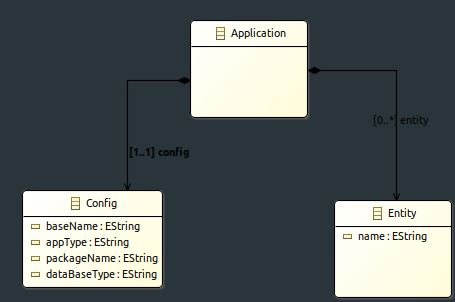
\includegraphics[width=16cm]{mmJdl.png}}
%       \caption{}
%   \end{center}
% \end{figure}

\subsection{Description du meta-model YAML}

La figure suivante présente un diagramme de classe décrivant 
le meta Model du YAML:

Aussi pour YAML:\\
\begin{figure}[H]
  \begin{center}
      \fbox{
      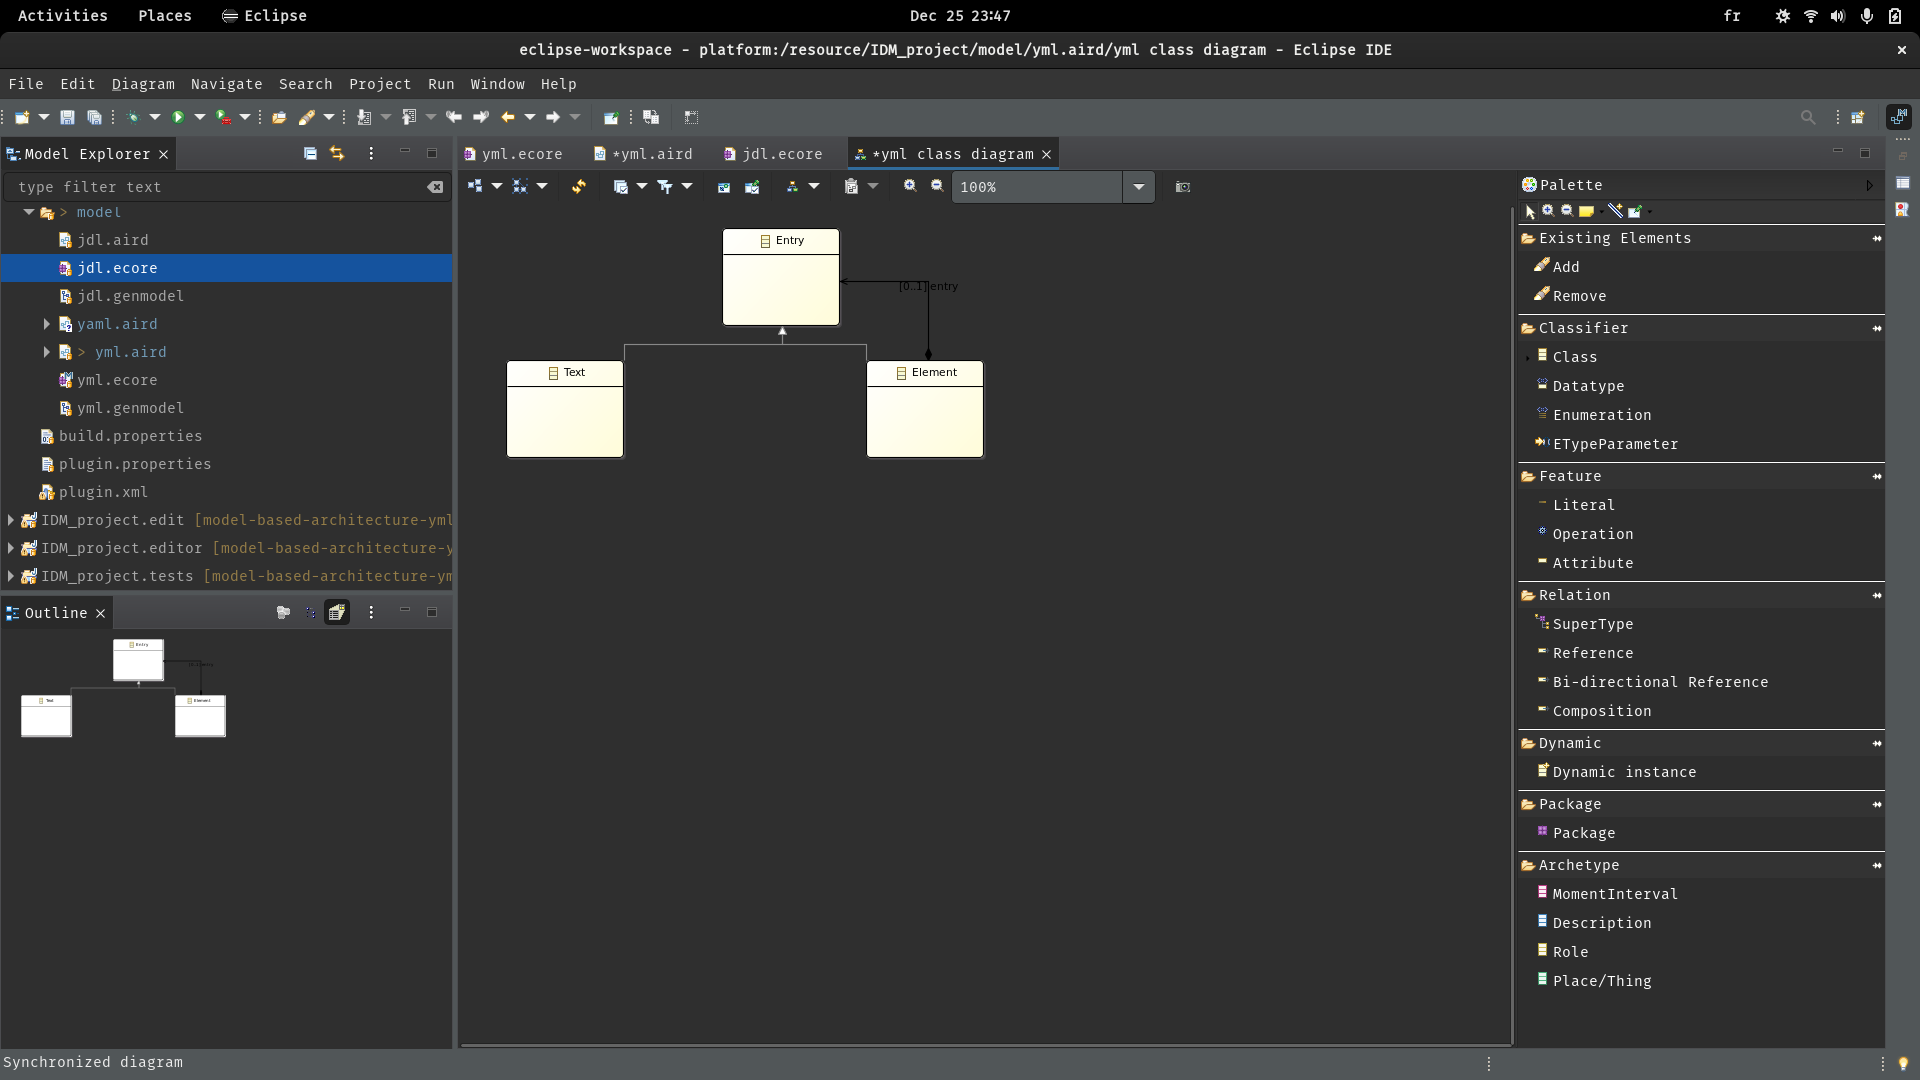
\includegraphics[width=16cm]{eclipse_yaml.png}
      }
      \caption{}
  \end{center}
\end{figure}	

\chapter*{Description des entrées, des transformations et des sorties}
\fancyhead[L]{\textbf{Chapitre: Description des entrées, des transformations et des sorties}}
\fancyhead[R]{\hspace*{5cm}}
%\section{Réalisation et gestion du projet}

\section{Description des entrées sorties}

Dans ce projet nous avons rencontré trois termes principaux: T2M, M2M,
M2T.

La transformation text-à-modèle est la première partie dans laquelle
on reçoit en entrée un fichier \texttt{.yml}. Il a la syntaxe normal
de \texttt{YAML} avec respect des régles définit en méta-modèle créé
auparavant. Cela se manifeste par l'utilisation des mots-clés définit
en \texttt{xtext} et inspirée du méta-modèles.

\begin{figure}[H]
  \begin{center}
      \fbox{
      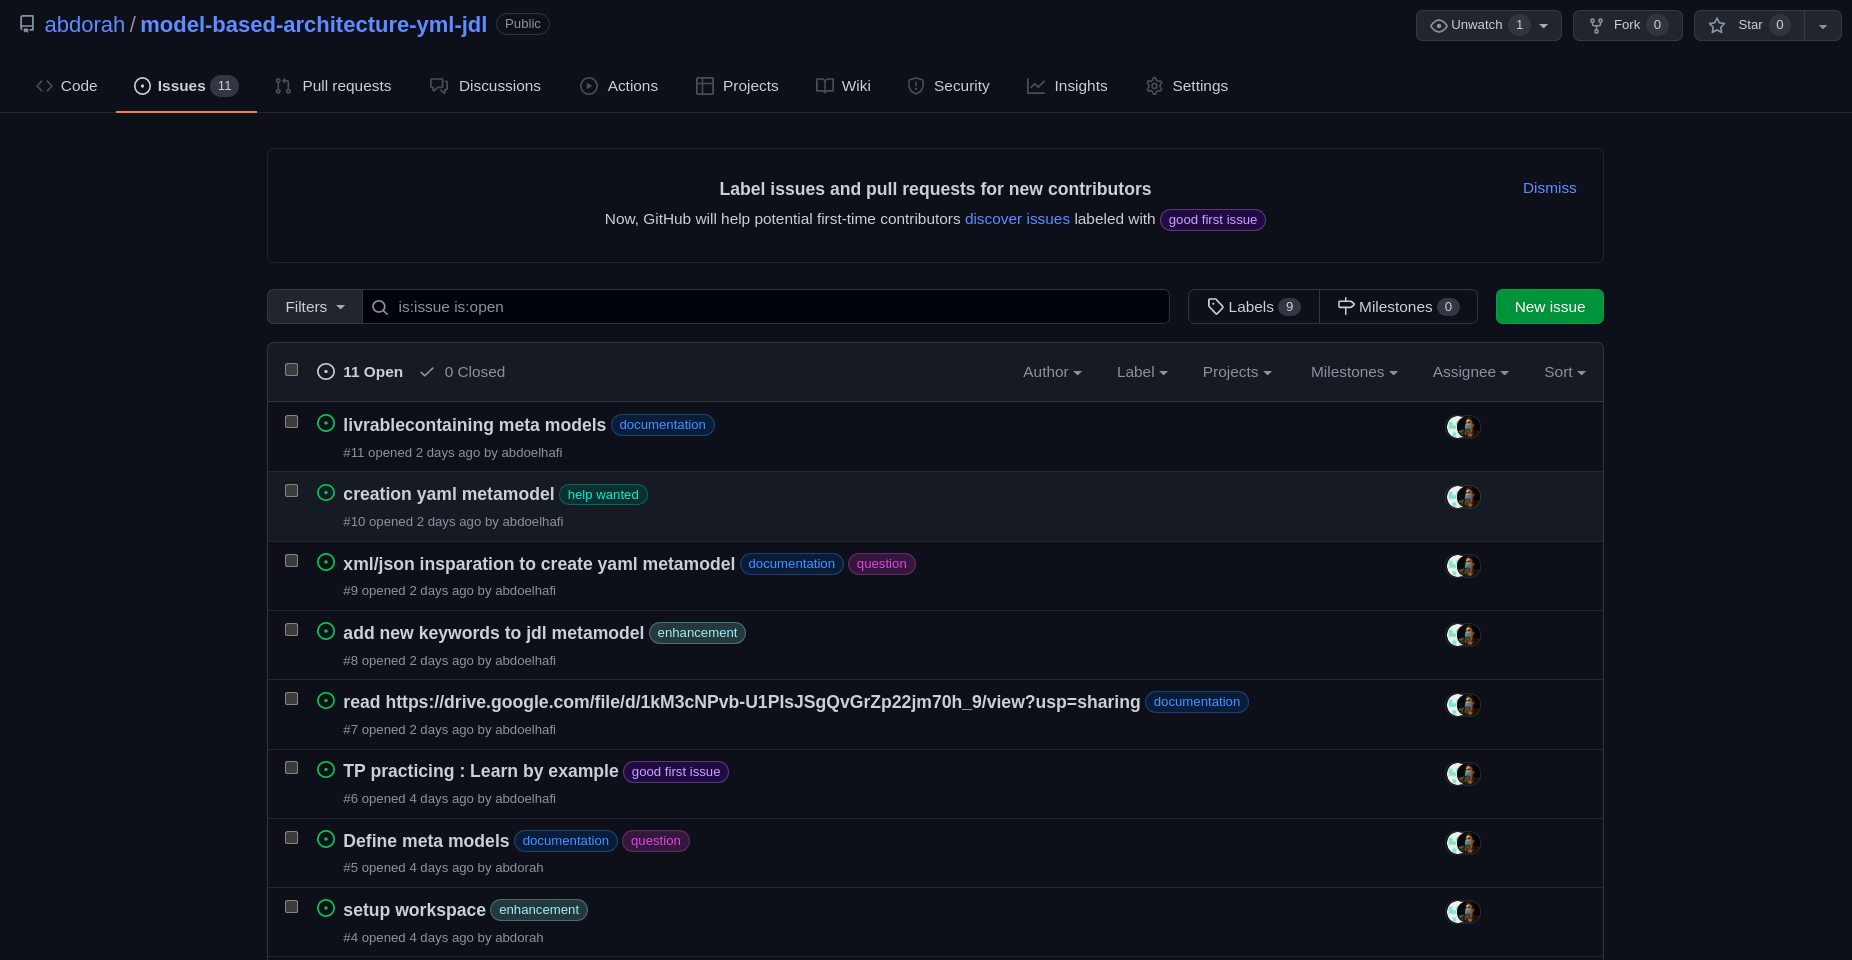
\includegraphics[width=16cm]{issues.png}
      }
      \caption{Les entrées de la transformation T2M}
  \end{center}
\end{figure}

L'étape qui suit est la transformation M2M. Cella, se fait en se
basant sur le modèle généré aprés la tranformation T2M. les deux
modèles générée sont des fichiers \texttt{XML}. L'outil de la
transformation utilisé est \texttt{ATL}. À la base du fichier
\texttt{main.atl}, où on a définit les régles de la transformation, on
génére le modèle \texttt{JDL}.

\begin{figure}[H]
  \begin{center}
      \fbox{
      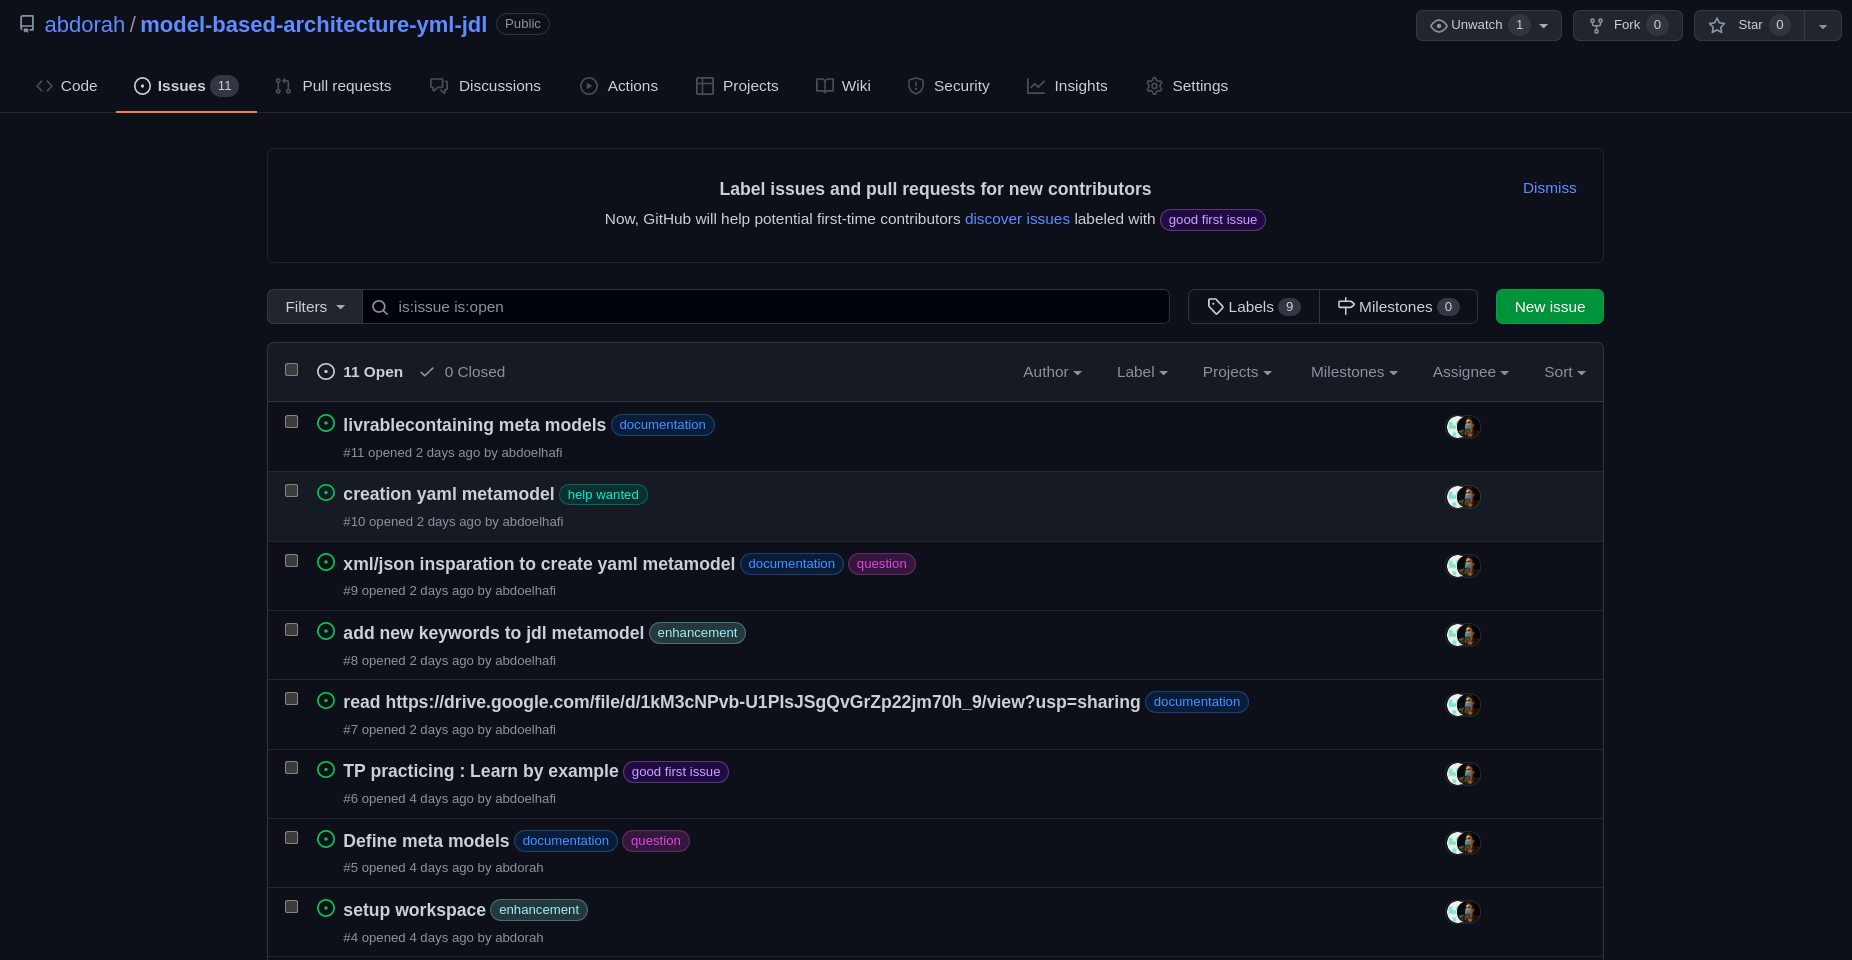
\includegraphics[width=16cm]{issues.png}
      }
      \caption{La transformation M2M}
  \end{center}
\end{figure}

Enfin, on arrive à effectuer un tranformation \texttt{M2T} en
utilisant \texttt{xtext} une autre fois. Ceci permet de générer un
fichier \texttt{.jdl}, réspectant la syntaxe de \texttt{JDL}.

\begin{figure}[H]
  \begin{center}
      \fbox{
      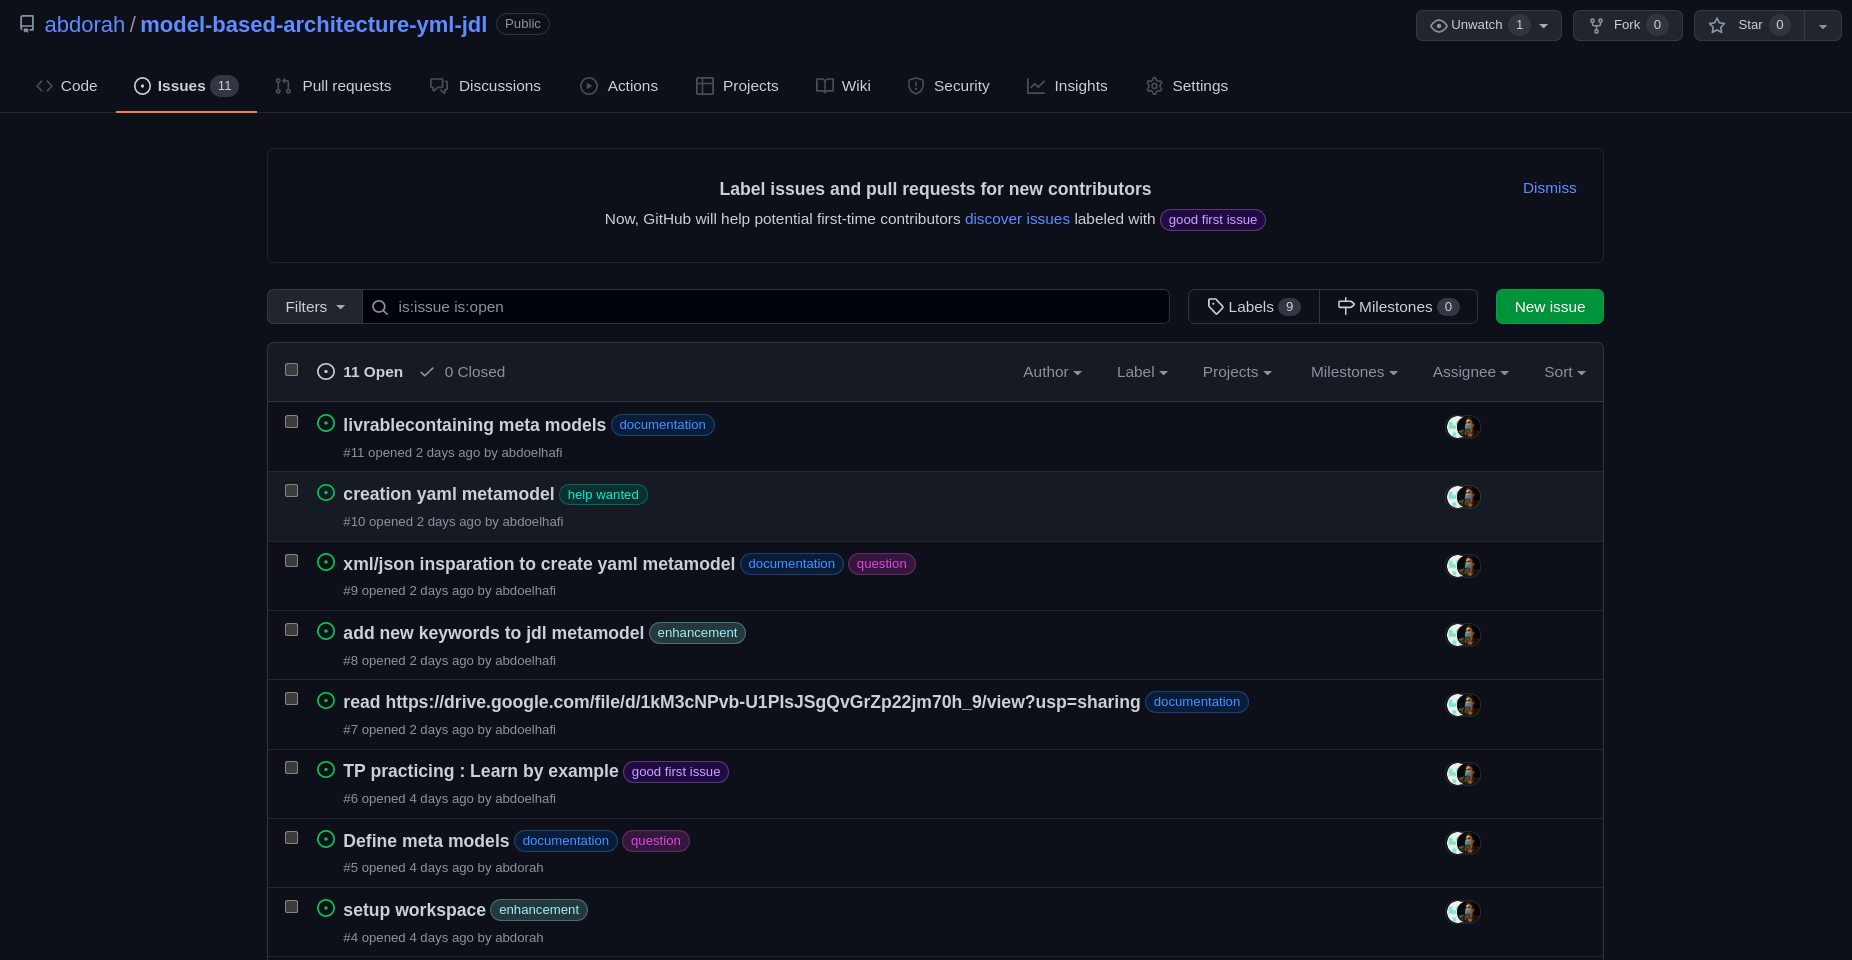
\includegraphics[width=16cm]{issues.png}
      }
      \caption{Les sorties de la transformation M2T}
  \end{center}
\end{figure}

\section{Mode de travail}

Il est primordial de bien gérer chaque projet et d'avoir une structure
claire et optimisée à suivre. Du coût, nous avons utiliser les outils
offers par la platforme Github pour la gestion de ce projet:

Chaque tâche est représenté par un "issue", quoi doit être assigné
manuallement à un memebre d'équipe:

\begin{figure}[H]
  \begin{center}
      \fbox{
      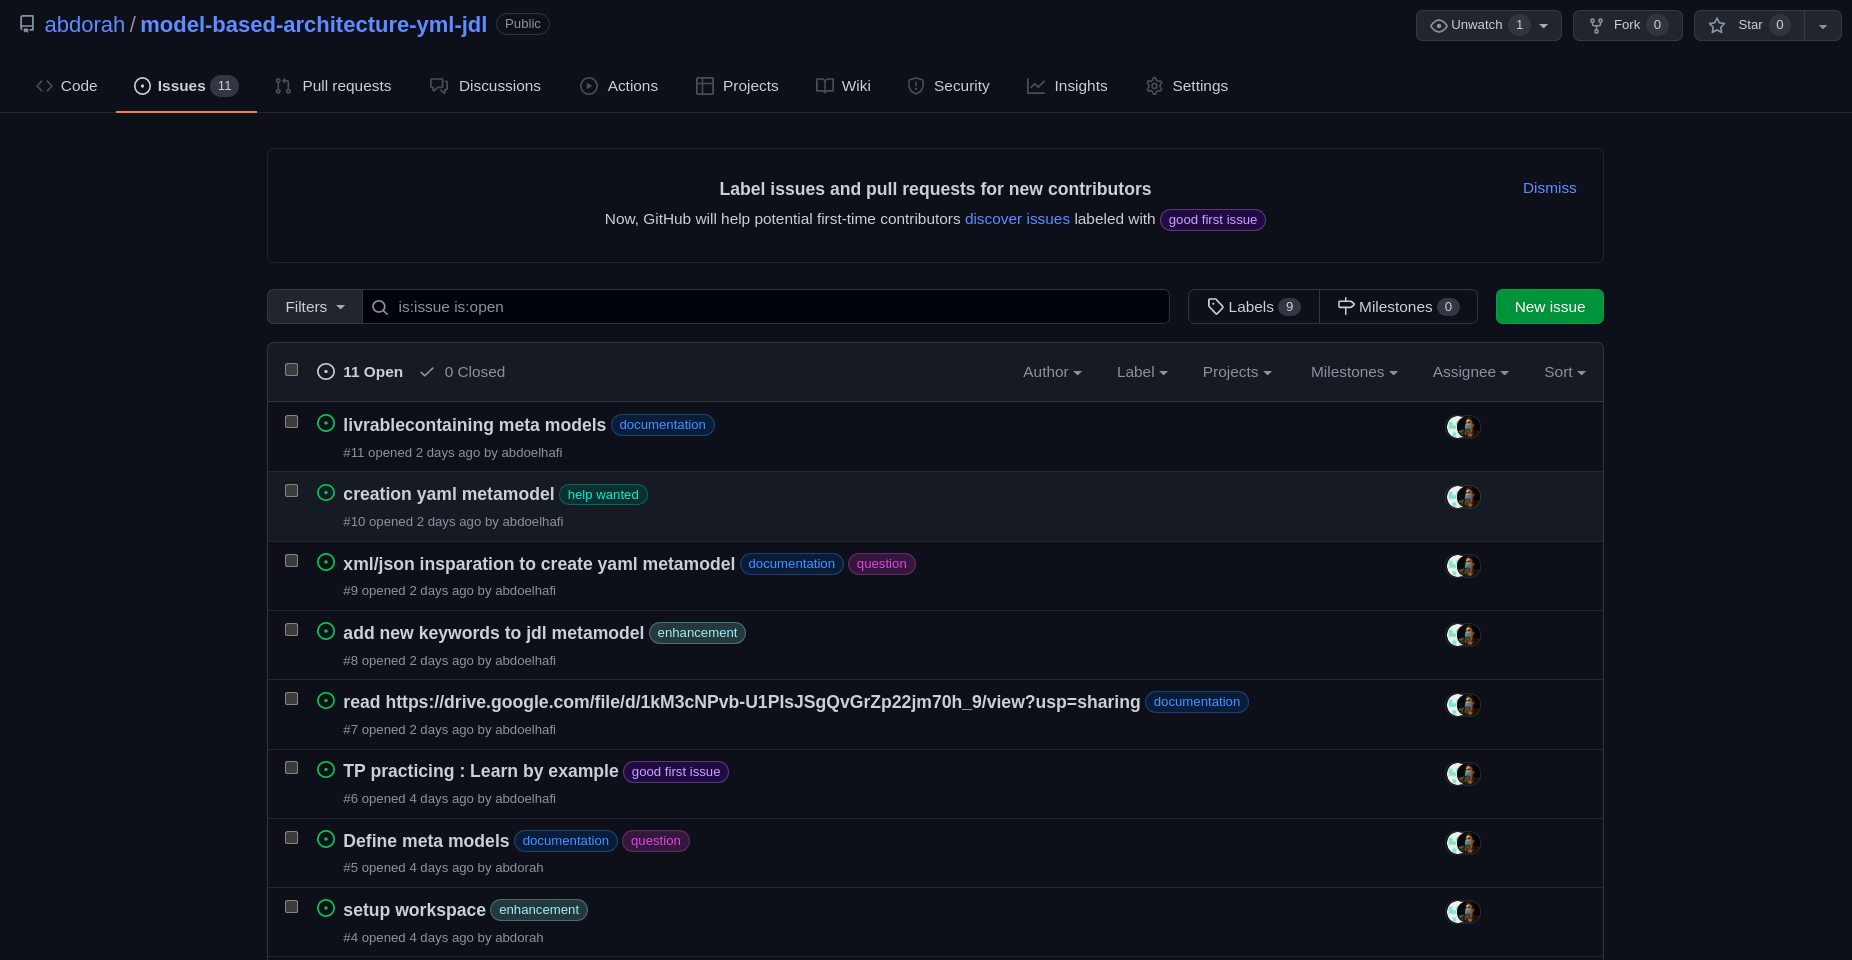
\includegraphics[width=16cm]{issues.png}
      }
      \caption{Liste des issues en Github}
  \end{center}
\end{figure}

Chaque issue est représenté par un ticket sur un tableau ayant la même
structure comme les tableux trello. Il contient touts les informations
necessaire sur le type, la définition, et l'état d'issue qu'en
concerne:

\begin{figure}[H]
  \begin{center}
      \fbox{
      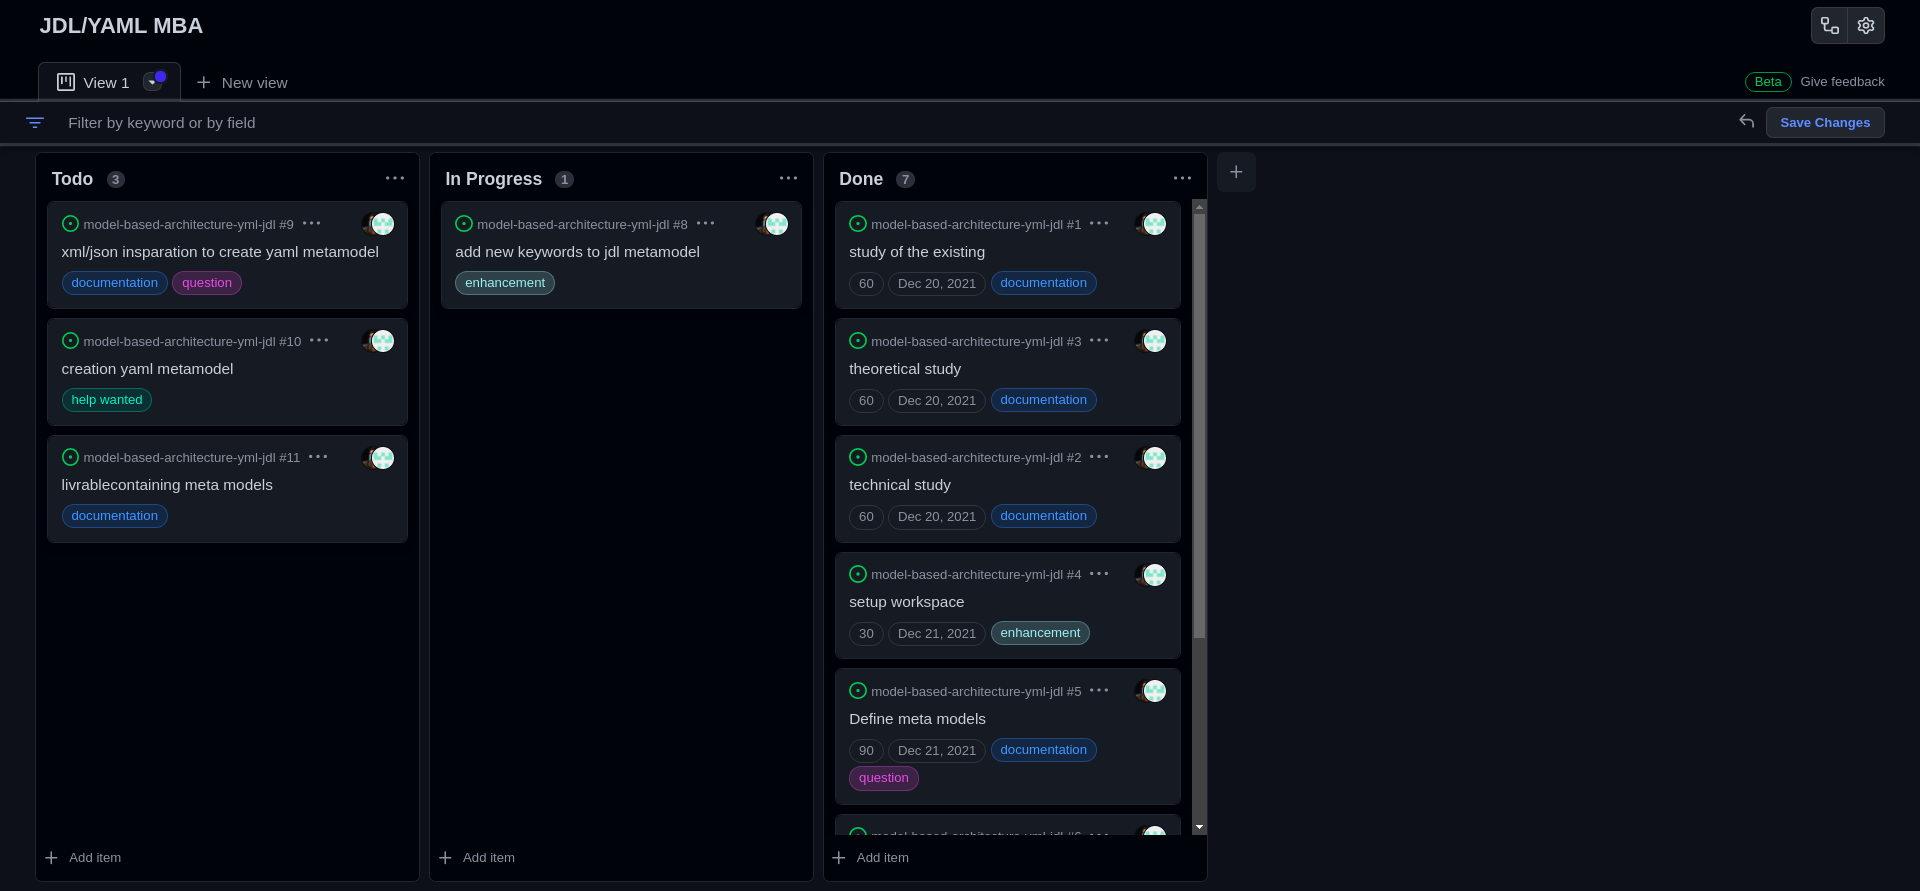
\includegraphics[width=16cm]{mode-trello.png}
      }
      \caption{Tableau Kanban pour la gestion des tâches}
  \end{center}
\end{figure}

Le modèle de tableau peut être représenté aussi sous-forme d'un tableau
contenant les mêmes informations d'une manières plus facile à
parcourir:

\begin{figure}[H]
  \begin{center}
      \fbox{
      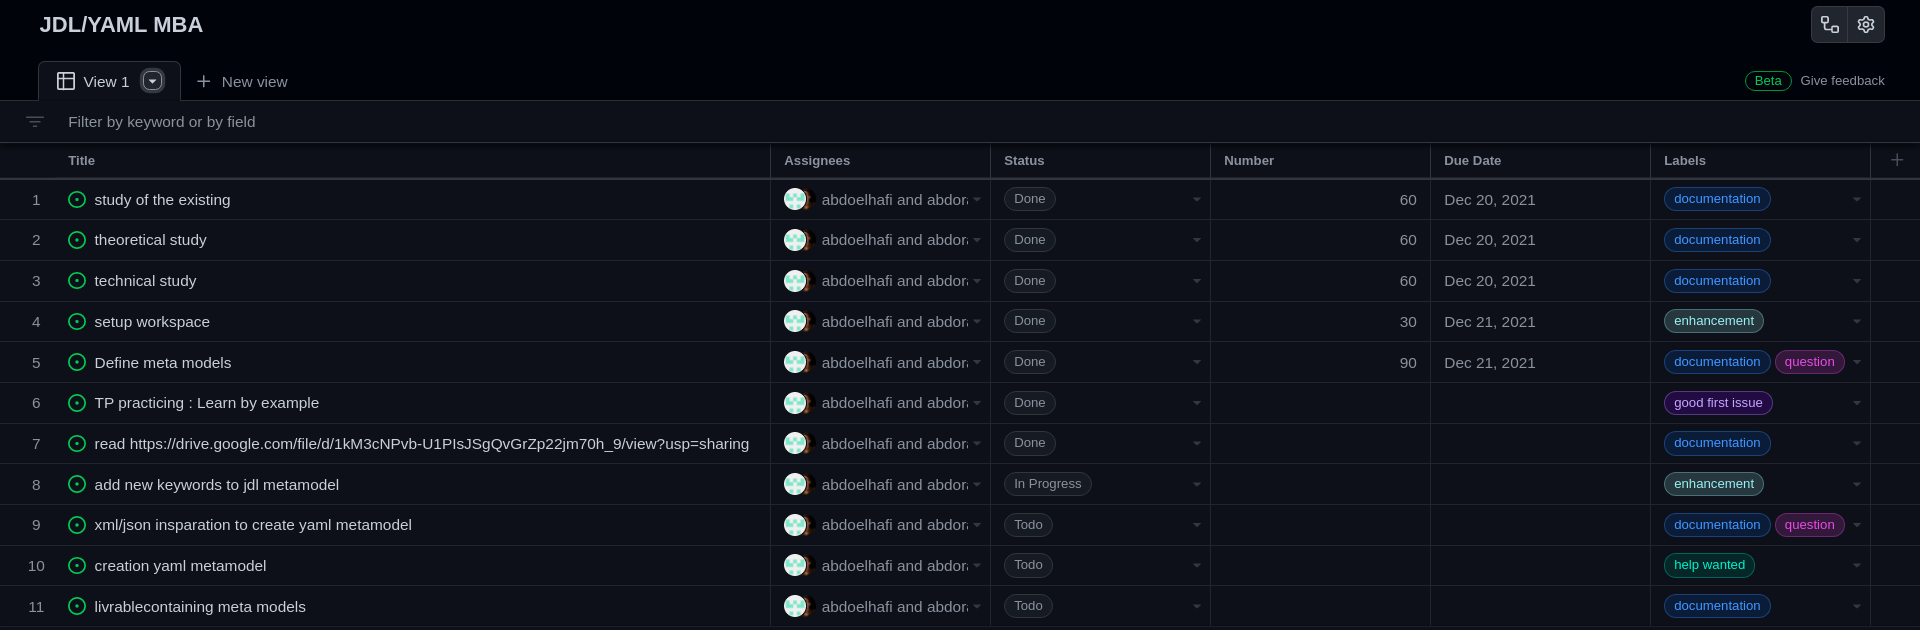
\includegraphics[width=16cm]{mode-table.png}
      }
      \caption{Tableau d'historiques des tâches}
  \end{center}
\end{figure}

Le cycle de vie d'un ticket dépend complétement de l'issue qu'en
concerne. Il se crée, prendre les dernières modification du issue, et
se label comme terminer si le issue est cloturé:

\begin{figure}[H]
  \begin{center}
      \fbox{
      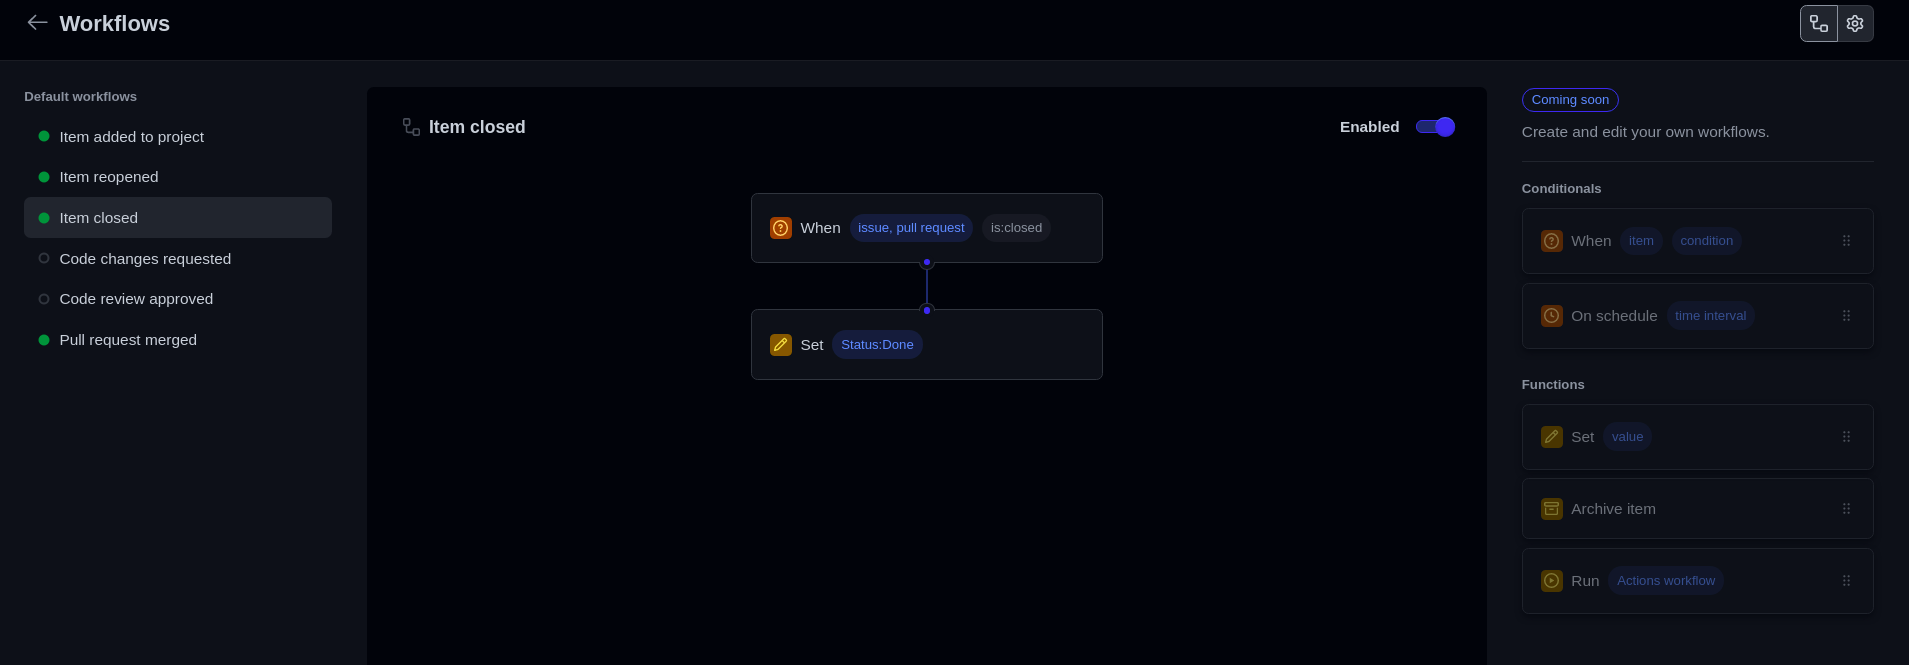
\includegraphics[width=16cm]{mode-automation.png}
      }
      \caption{Processus d'automation de la transformation des tâches en issues}
  \end{center}
\end{figure}

\section{Structure du projet}

La téchnologie utilisée dans ce projet est EMF. qui représente un
ensemble des outils trés puissants pour le MDSE.

Le projet à la structure suivante:

\begin{figure}[H]
  \begin{center}
      \fbox{
      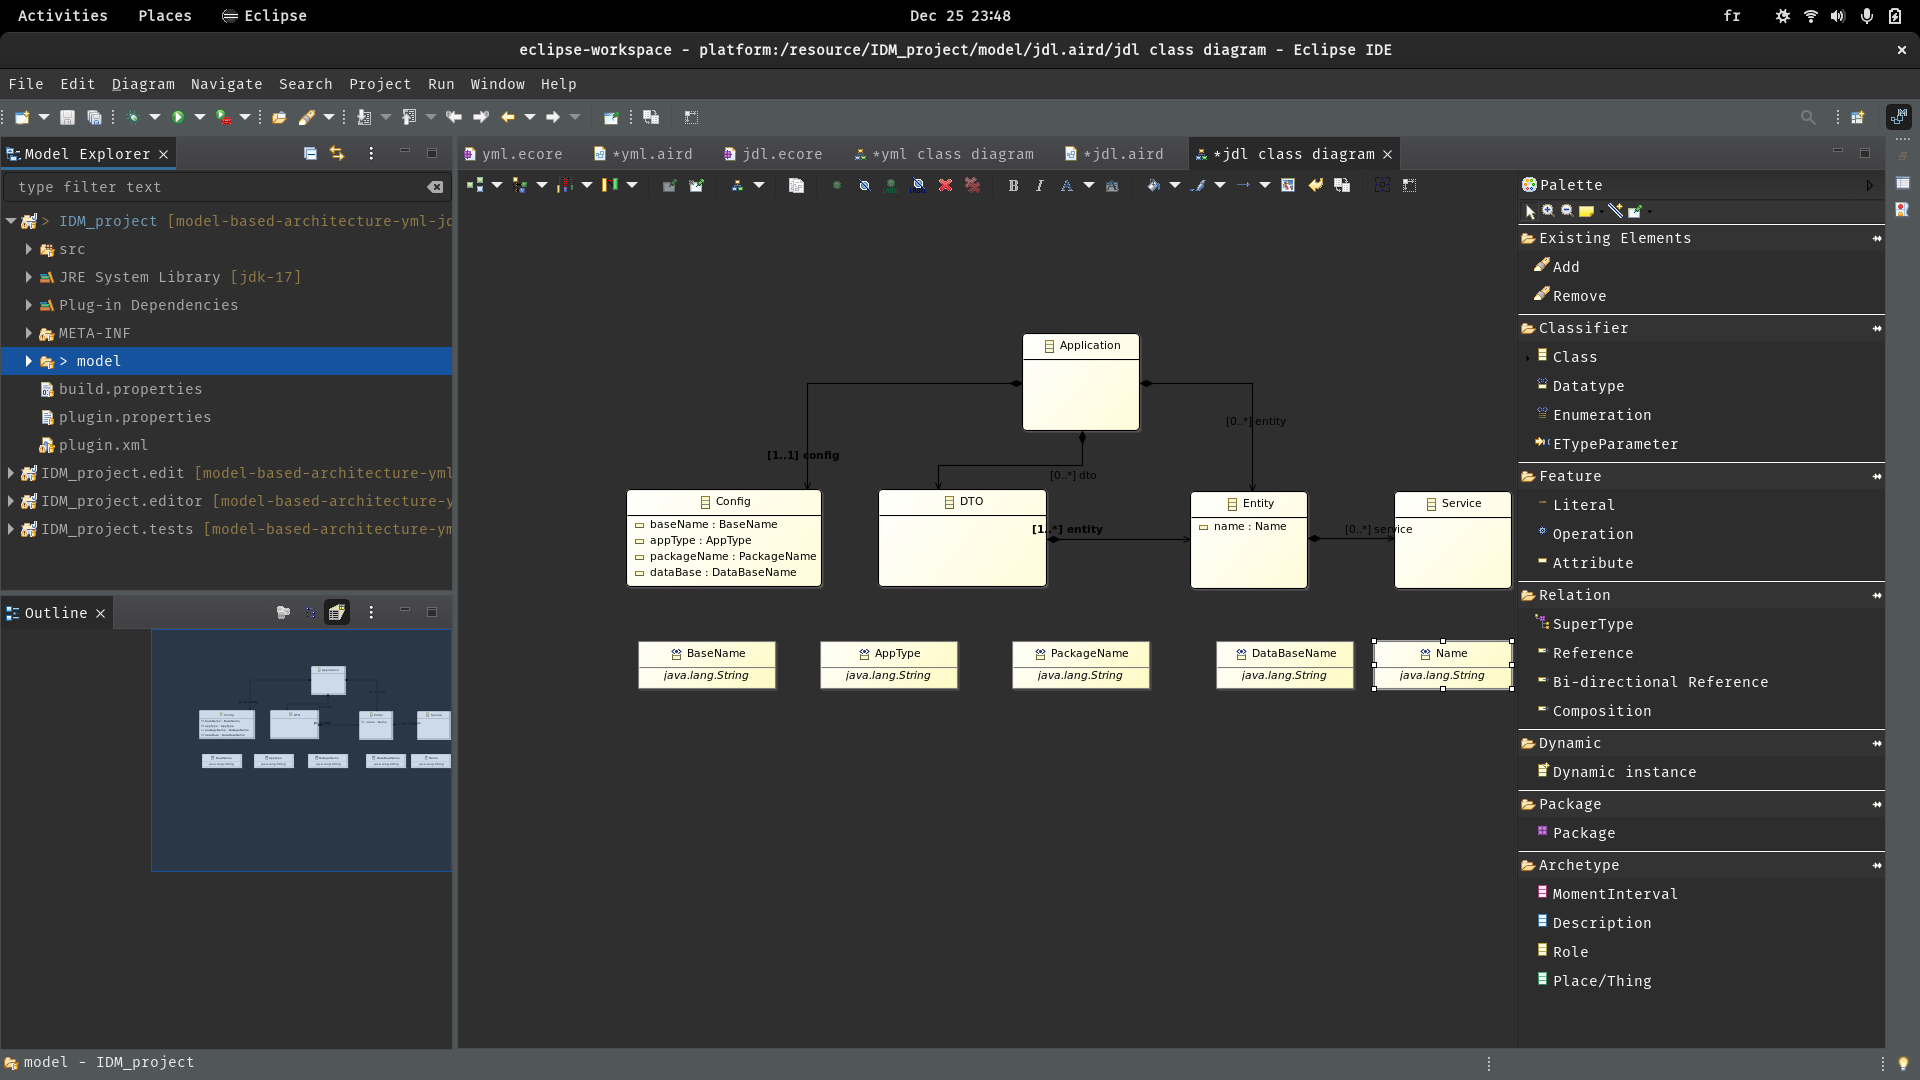
\includegraphics[width=16cm]{eclipse-jdl.png}
      }
      \caption{Diagramme des classes du méta-modèle de JDL}
  \end{center}
\end{figure}

Aussi pour YAML:

\begin{figure}[H]
  \begin{center}
      \fbox{
      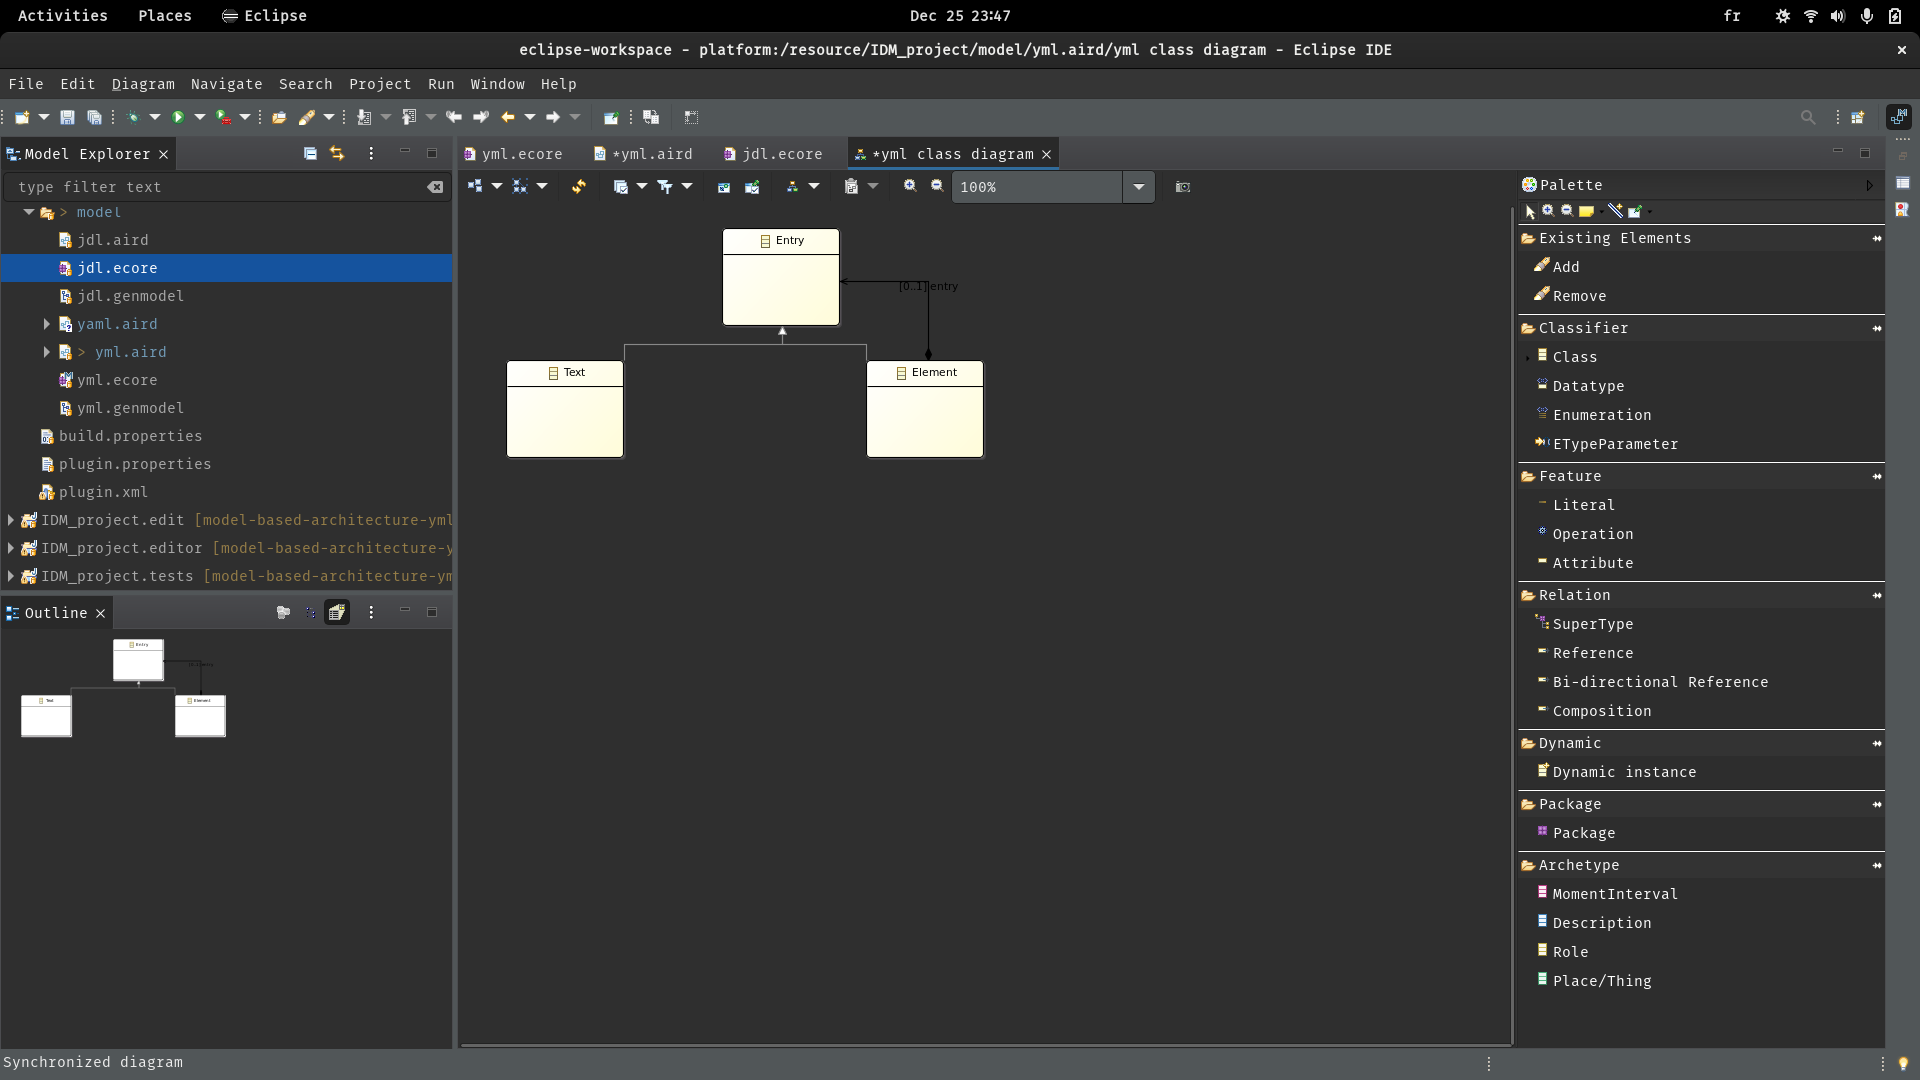
\includegraphics[width=16cm]{eclipse_yaml.png}
      }
      \caption{Diagramme des classes du méta-modèle de YAML}
  \end{center}
\end{figure}
	

\end{doublespace}

\end{document}
